\chapter{Qu'est ce que l'homme pour l'Islam ?}
\mn{Delphine Ortis \newline Chercheur(e) indépendant Ethnologie / Anthropologie sociale
Delphine.ortis@gmail.com}
\section{Approche et validation}

\paragraph{Approche}
\begin{itemize}
\item diversité de l'islam
\item dignité de l'homme
\item figures d'autorité : 
\begin{itemize}
\item le prophète et le Sunnisme
\item l'\imam dans le Chiisme
\item le Saint dans le soufisme
\end{itemize}
\item Eschatologie
\end{itemize}

\paragraph{Validation du Cours}Présenter un support de cours et partager un thème sur l'article sur 2 pages et on le présente : 
\begin{itemize}
\item Revue des Mondes Musulmans et de la Méditerranée\sn{\href{https://journals.openedition.org/remmm/}{RMMM}}
\item Revue de l'extrême orient
\end{itemize}
Résumé de l'article. On situe l'auteur. C'est quoi son sujet ? Qu'est ce qu'il a voulu démontré ? Comment ? 
Commentaire personnel 


\chapter{Diversité de l'Islam}

On pense au sunnisme. il faut penser aux sectes, les séparations religieuses mais il y a aussi les différences culturelles.
\paragraph{Des schismes à la mort du Prophète} Sans fils et sans testament, la succession de Mohammed est problématique. Les Califes sont ses compagnons de la même tribu et même souvent à son clan. 

\subparagraph{les Califes bien dirigés} Les premiers califes sont des compagnons mais ne sont pas des \textit{ gens de la maison}.
 
\subparagraph{Fatima, seule enfant du prophète} épouse Ali, le cousin germain du prophète. Seuls eux sont \textit{gens de la maison}

\subparagraph{Uthman} 3eme calife est assassiné en 655. Du coup, séparation entre trois groupes après la bataille de \textit{Siffin} (657) : 

\begin{itemize}
\item Sunnites : 87,4\%
\item Chiites : 11,9\%
\item Kharijites : 0.7\% (Ibadisme en Oman), les \textit{séparés}
\end{itemize}

Ces trois groupes vont élaborer des doctrines différentes sur le califat.

\paragraph{Les inégalités reconnues dans l'Islam}
Au nombre de trois :  
\begin{itemize}
\item Croyant / non Croyant
\item homme / femme
\item homme libre / esclave (écrit dans le Coran)
\end{itemize}
Dans les croyants, on peut mettre les gens du livre. 

\paragraph{Le Sunnisme et ses 4 écoles juridiques}
\subsection{les écoles Juridiques}
\begin{figure}
    \centering
    \sidecaption{Atlas de l'Islam dans le monde, Anne Laure Dupont, Autrement, 2005}
    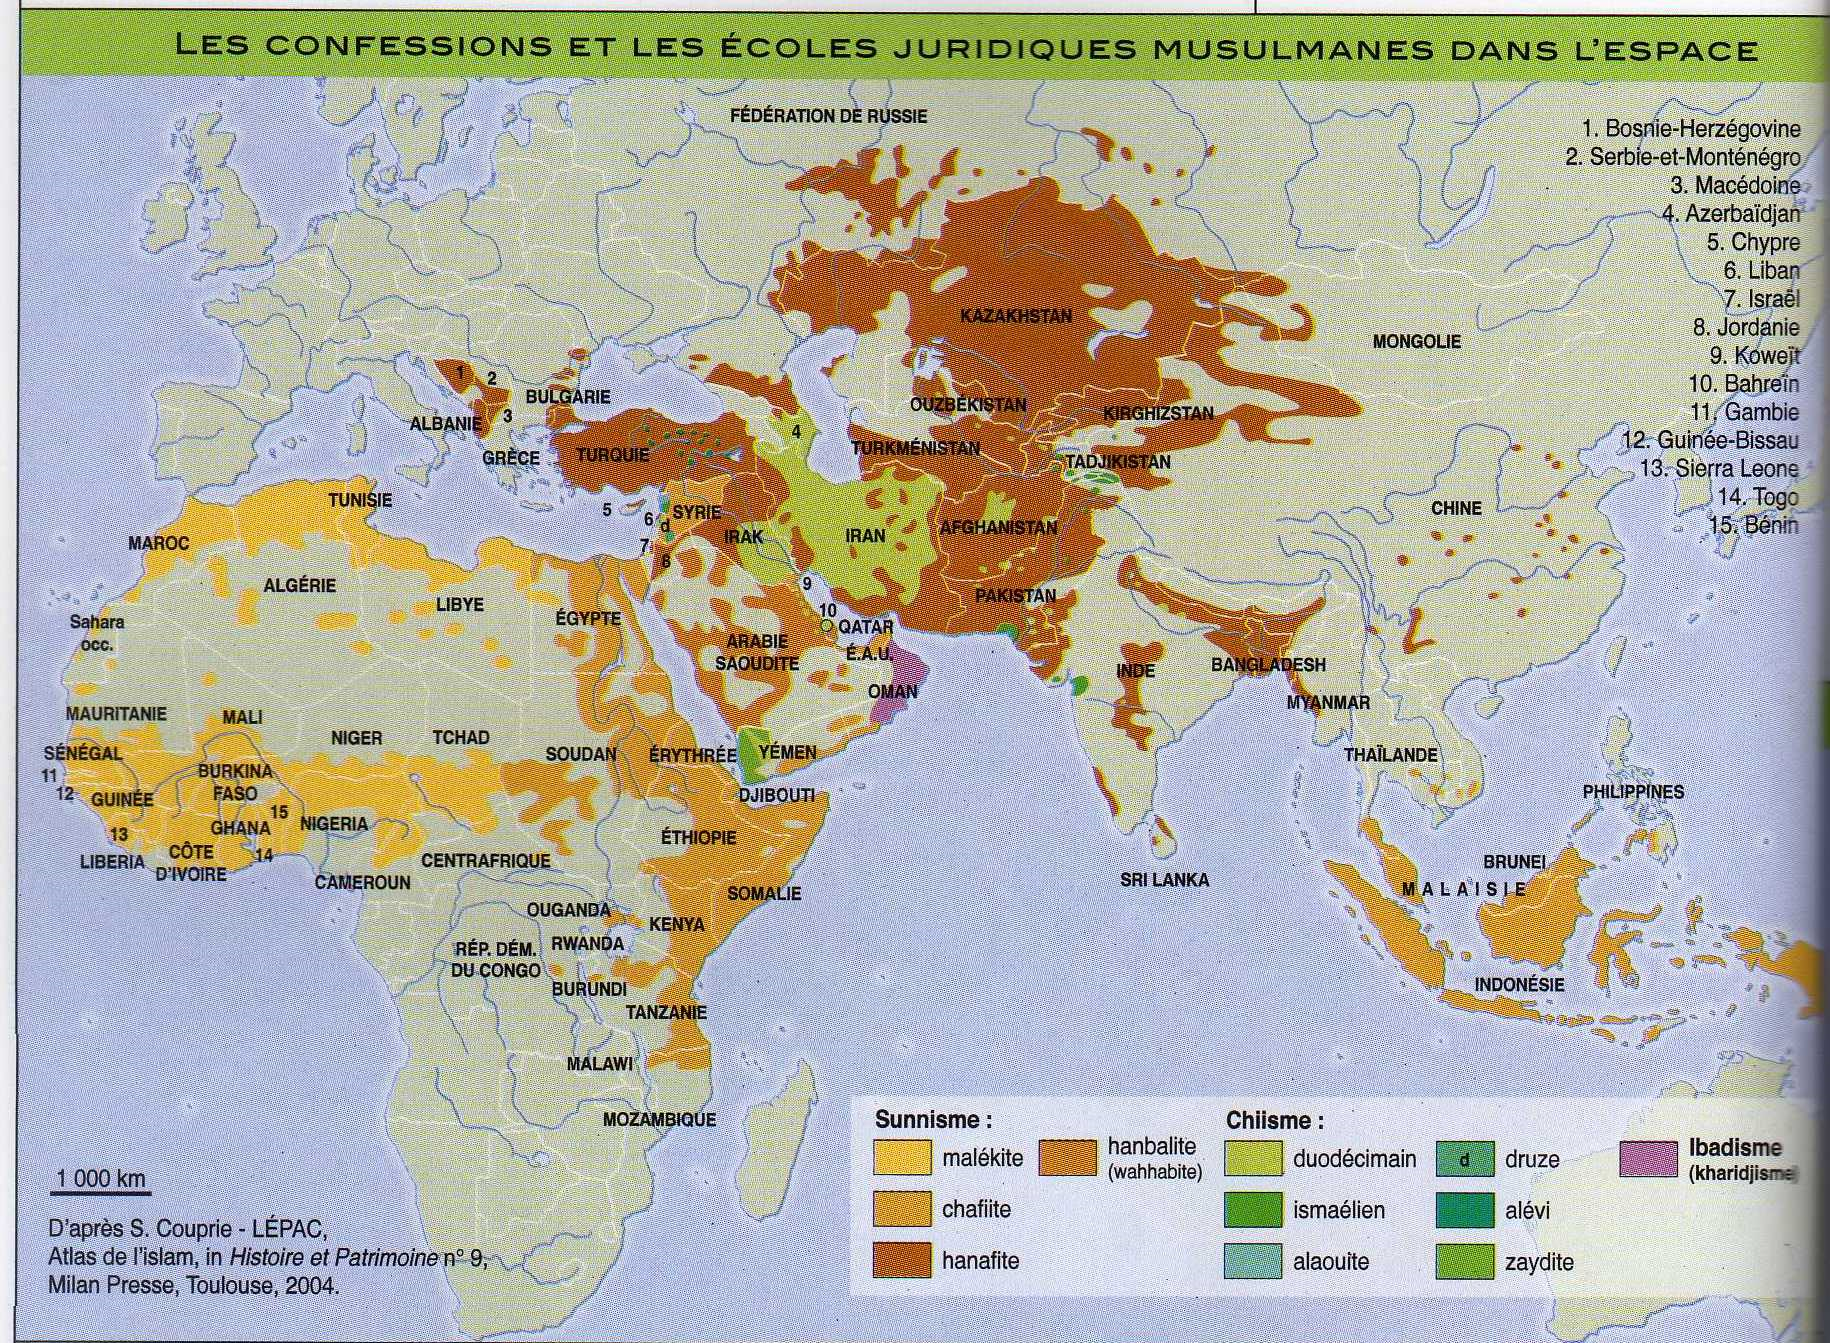
\includegraphics[width=\textwidth]{CourantsIslamContemporain/ImagesCourantsIslamContemporain/CarteSunnisme.png}
 
    \label{fig:my_label}
\end{figure}



\bi 
\item  malékisme : Afrique Nord et ouest.
\item Chafiite : Est de l'Afrique et surtout Egypte 
\item Hanafite : Turquie, asie Centrale, Inde. \textit{les empires turques}
\item Hanbalite : surtout Arabie Saoudite, transformé en \textit{Wahhabisme} au XX, avec une extension au dela de l'Arabie Saoudite en 1960.
\ei 

\paragraph{Les Kharijites} même un esclave noir peut devenir Calife\mn{Dans le désert Algérien, on trouve des kharijites}. En disant cela, les kharijites sinsistent sur l'individu. On le juge juste sur son discours. 
Ce groupe se scinde : 
\begin{itemize}
\item Ibadite (Zanzibar et Oman). Il se caractérise par un très fort égalitarisme et une rigueur morale.
\item autres ? 
\end{itemize}

\paragraph{Le Chiisme} Les chiites insistent sur le fait que les califes doivent être des \textit{gens de la maison}, Ali et ses descendants. Le premier \imam est Ali, puis Hassan, puis Husayn. On arrive au 6ème \imam Jafar al Sadiq. Il désigne Ismael, son fils ainé, qui décède avant son père. Comme Jafar n'a pas nommé de successeur, la communauté chiite se scinde en différents courants : 
\begin{itemize}
\item les Ismaeliens ou septimains (7 imams, l'Aga Khan), Liban. Ismael n'est pas mort, dans une sorte d'occultation. Il réapparaitra à la fin du temps.  
\item Les duodécimains (ils reconnaissent 12 imams) : les shi'ites Iraniens: disent que le successeur est \textit{Musa}, le second fils de Jafar. Le \textit{Mahdi} est le douzième \imam, Mohammed al-Madhi.
\item zaydites (5 imams) : Yemen. Au niveau de la doctrine, ils reconnaissent peu de pouvoirs divins aux \imam  (proches des Sunnites de ce point de vue).
\end{itemize}


\begin{Synthesis}[divergence en Si'isme : les courants]
Des désaccords sur Qui est \imam et sur la \textit{nature de l'Imam}. Il peut être investi de pouvoirs divins.
\end{Synthesis}

\begin{Def}[Mahdi]
Le Mahdi, celui qui revient à la fin des temps et qui va lutter avec Jésus contre l'armée du mal :
\begin{itemize}
\item Il n'est pas né
\item pour les septimains, c'est \textit{Ismael}, qui n'est pas mort
\item pour les duodécimains, c'est le 12ème \imam
\end{itemize}
\end{Def}
